\subsubsection{Oceanic extension}
\label{sec:cookbooks-oceanic-extension}
\textit{This section was contributed by Valentina Magni, John Naliboff, and Anne Glerum}

This cookbook shows how to build a model of oceanic lithosphere extension, starting from a simple setup and adding complexities step by step. In all models we simulate extension by imposing outflow at the side boundaries and observe how the oceanic lithosphere deforms with different rheologies. 
(VM - Maybe add here a brief description of all the steps)
(VM - I will need to add a. section of solver schemes when the other models are done)

\paragraph{Reference model setup}
In the first model, we start with solely oceanic lithosphere, we will add the asthenosphere in a later step. In the reference model, we use a 2D Cartesian geometry with a computational domain that is 400 km long (x-direction) and 100 km deep (y-direction). The mesh is refined globally to 5 levels (128x32 elements). An additional level of mesh refinement is implemented in the shallow central part of the box (above 50 km and between 120 and 280 km) because this is where we expect deformation to occur. Therefore, the grid in this area has a resolution of 1.56 km (Fig.~\ref{fig:figure_initial_setup}).

\lstinputlisting[language=prmfile]{cookbooks/oceanic_extension/doc/oceanic_extension_geometry_mesh.prm.out}


Now we need to specify the initial composition and temperature field that describe an oceanic plate. We use compositional fields to track the oceanic crust and lithospheric mantle during the model evolution. In the list of fields, we also need a field for plastic strain, which keeps track of strain accumulated during brittle (plastic) deformation. 
The initial values of plastic strain are computed using the function rand\_seed that creates a random field that is reproducible by giving a specific integer number as an input. Here, for example, we use rand\_seed(0), but one can test different initial random fields, by changing the number within parenthesis. We impose this random values of plastic strain in the central part of the model, where we want deformation to localise. Although we know that these values are important to localise deformation only above the brittle-ductile transition, we impose this random field of plastic strain values over the entire height of the domain, to make sure we resolve the brittle-ductile transition if/when we change the age of the plate (thus, its geotherm). The second compositional field is the oceanic crust, which is initially 7 km thick, and below the lithospheric mantle, untile the bottom of the box (Fig.~\ref{fig:figure_initial_setup}).

\lstinputlisting[language=prmfile]{cookbooks/oceanic_extension/doc/oceanic_extension_composition.prm.out}


The initial temperature field follows the plate cooling model for a 40 Myr old oceanic plate, assuming a mantle temperature of 1573 K and a thermal diffusivity of 1.0101e-6 m\textsuperscript{2}s\textsuperscript{-1}. The value of thermal diffusivity is consistent with values of thermal conductivity, heat capacity and density used in the material model further down in the parameter file.

\lstinputlisting[language=prmfile]{cookbooks/oceanic_extension/doc/oceanic_extension_temperature.prm.out}


\paragraph{Boundary conditions}
As described above, we simulate extension by using outflow boundary conditions at the sides. This is done by imposing prescribed boundary conditions for the x-component of the left (-0.5 cm/yr) and right (0.5 cm/r) boundaries. Therefore, the total extension rate is 1 cm/yr. The bottom boundary is free-slip and the top has a free surface. The surface velocity projection set to "normal" allows for the free surface to be advected both vertically and horizontally, which provides a more realistic approximation of the topography evolution, compared to the option "vertical" that would advect the surface only vertically. Note that with these boundary conditions, the model loses mass over time because there is no inflow of new material. Therefore, this model cannot be run for a long time. Here, we chose to run it until it reaches 2 Myr. 
For the temperature boundary conditions, we prescribe fixed values at the top and bottom. We use a function that assigns 273 K at the top and, at the bottom, the temperature computed for a 40 Myr old oceanic plate. For this, we use the same expression that describes the initial temperature field, but computed only at 100 km of depth. 
Finally, because there are no inflow boundaries, we do not need to specify anything for the boundary conditions of the compositional fields.

\lstinputlisting[language=prmfile]{cookbooks/oceanic_extension/doc/oceanic_extension_boundary_conditions.prm.out}


\begin{figure}
\centering
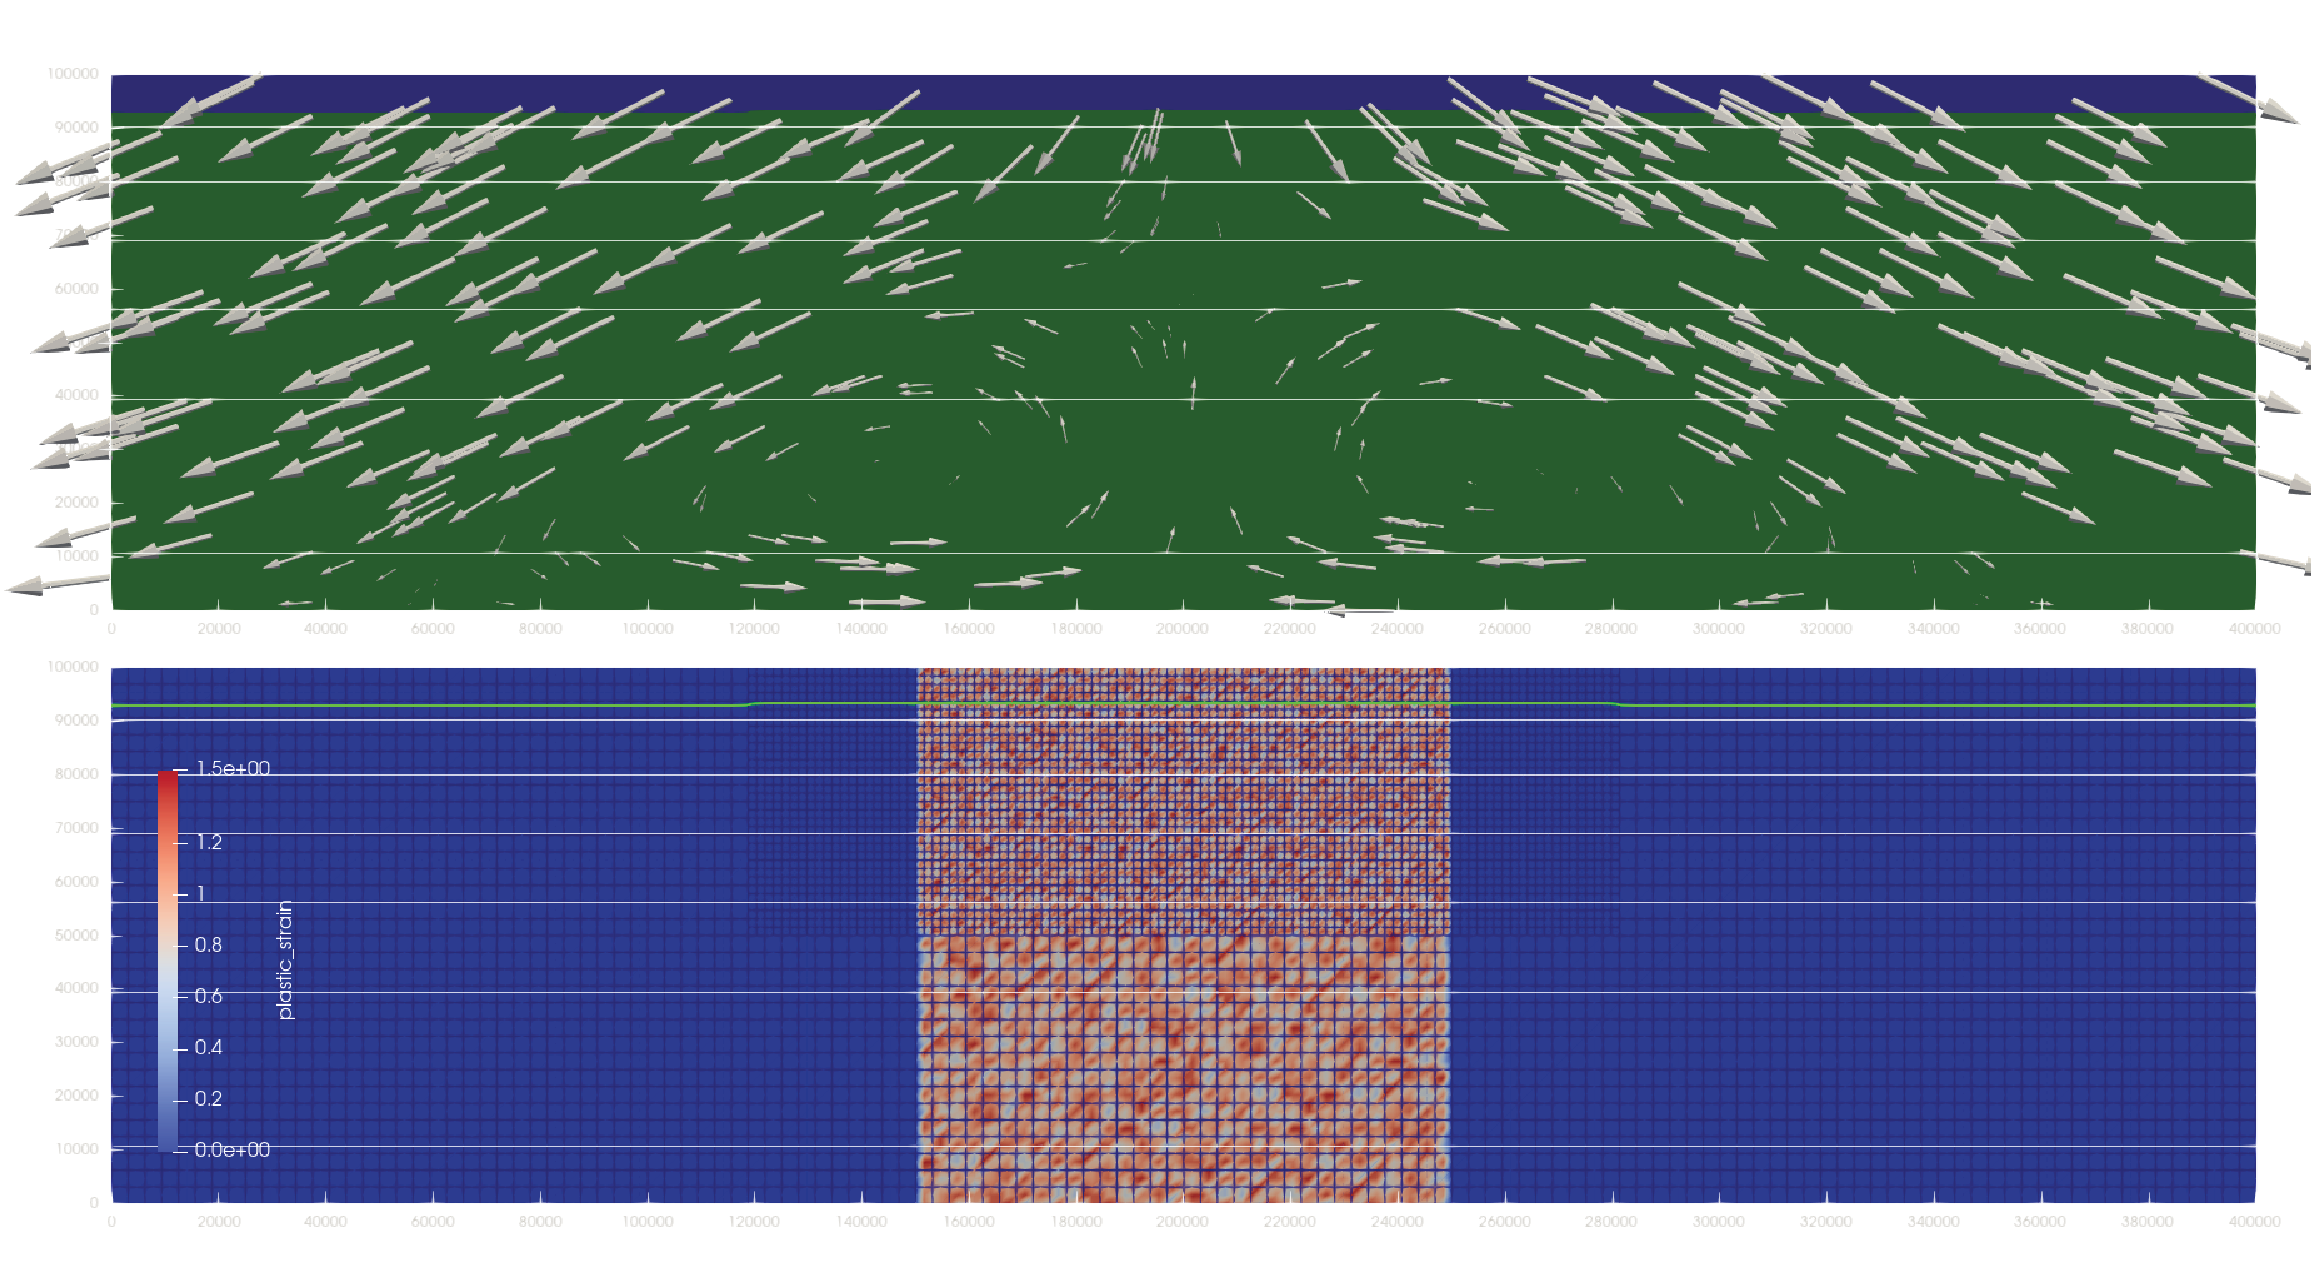
\includegraphics[width=\textwidth]{cookbooks/oceanic_extension/doc/figure_initial_setup.png}
\caption{\it Initial model setup. Top panel: compositional fields of oceanic crust (blue) and lithospheric mantle (green) and velocity field at time step 0. Bottom panel: initial random values of plastic strain and mesh. Isotherms are shown in white each 200 $\degree C$.}
\label{fig:figure_initial_setup}
\end{figure}

\paragraph{Rheology}
To model lithospheric deformation, we use a visco-plastic rheology, which takes into account both brittle and viscous deformation. To do that, we use the material model "visco plastic" and the viscous flow law "composite". In this way, the viscosity for each deformation mechanism (i.e, Drucker Prager yielding, diffusion creep, and dislocation creep) will be computed in each point of the grid and the lowest value will be used as effective viscosity. We define values of flow laws for diffusion and dislocation creep for each compositional field: gabbro flow law for the oceanic crust (Wilks and Carter, 1990) and dry olivine for the lithospheric mantle (Hirth and Kholstedt, 2003). Because we also use a compositional field for plastic strain, we need to define values also for this field. We set these parameters to values that give an unrealistic high viscosity, so that they will not be used to compute the effective viscosity. 
In addition to the deformation mechanisms described above, we also allow for strain weakening. In this model, plastic weakening depends only on plastic strain. This is where we use the plastic strain compositional field that we defined before. By setting weakening factors to 0.5, friction and cohesion will be lowered by factor 2 between plastic strain values of 0.5 and 1.5 (these are also parameters that can be set). Therefore, when we defined a random values of plastic strain in the central region of the model, we also changed the friction and viscosity values compared to their reference value. This helps to localise deformation and forming faults-like structures. Higher values of weakening factors will reduce less the viscosity, whereas lower values will have a higher impact on decreasing the viscosity through the brittle deformation mechanism. 
An other thing worth noting is that we use an harmonic average scheme for the way material properties are averaged over the grid. This allows for a smooth and stable solution, but does create less sharp contrasts at the interface between different materials. 
(VM - Maybe no need to add the entire material model, only some parts?)

\lstinputlisting[language=prmfile]{cookbooks/oceanic_extension/doc/oceanic_extension_material_model.prm.out}

\paragraph{Model dynamics}
Oceanic lithosphere starts to deform in the central area, which is characterised by the largest amount of subsidence. After 2 Myr of continuous extension, we can observe a graben structure in the central area bounded by normal faults. These fault-like structures are clearly visible in the plastic strain and strain rate fields, which show where most of the deformation occurred (Fig.~\ref{fig:figure_2Myr}).

\begin{figure}
\centering
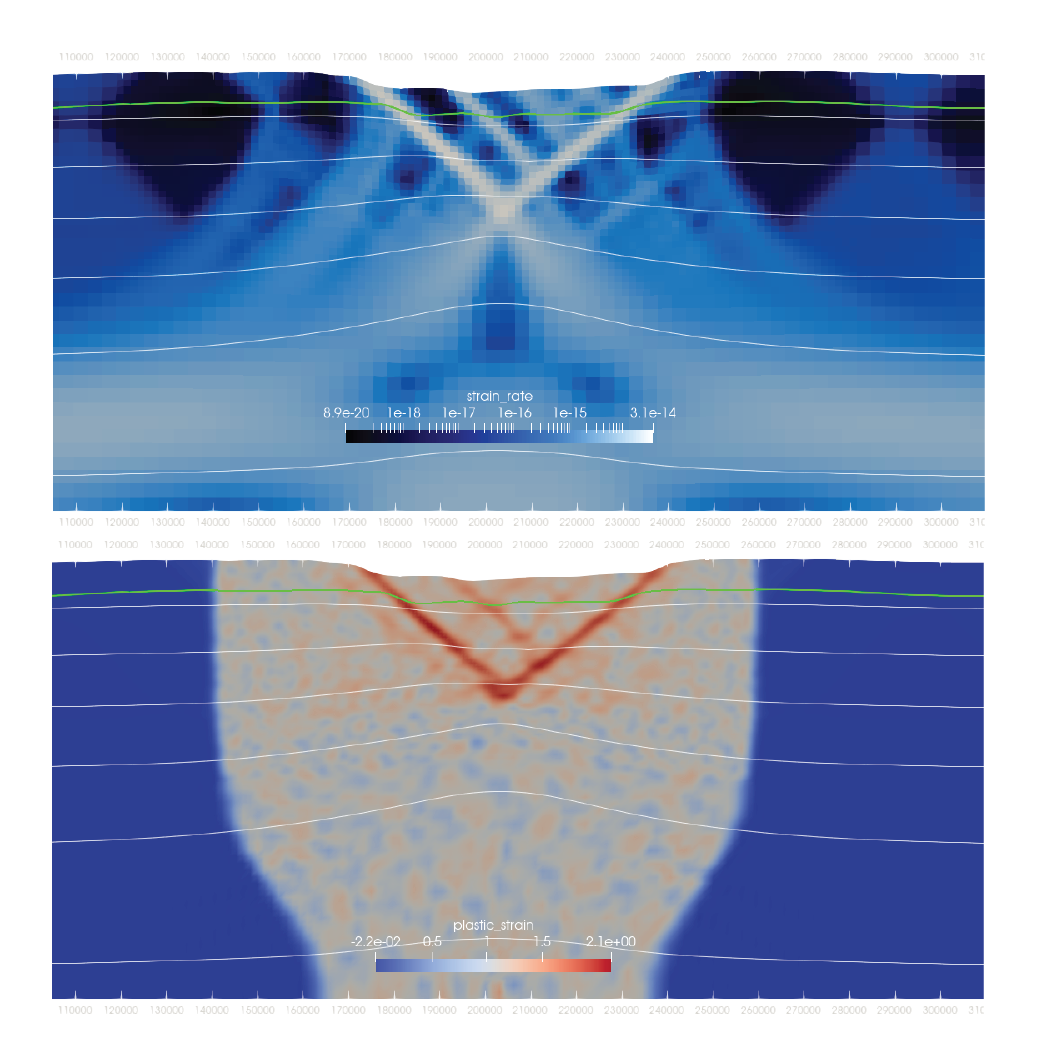
\includegraphics[width=\textwidth]{cookbooks/oceanic_extension/doc/figure_2Myr.png}
\caption{\it Strain rate (top panel) and plastic strain (bottom panel) after 2 Myr of extension at a rate of 1 cm/yr. Green line shows the bottom of the oceanic crust. Isotherms are shown in white each 200 $\degree C$.}
\label{fig:figure_2Myr}
\end{figure}



